\documentclass[11pt]{article}

% arXiv version. Self-contained: figures live in figs/.
% Build: tectonic main.tex   (or pdflatex main.tex twice)
% Numbers: compute_stats.py -> report/stats.json; verify_claims.py -> report/claims.json

\usepackage[margin=1in]{geometry}
\usepackage[T1]{fontenc}
\usepackage{lmodern}
\usepackage{graphicx}
\usepackage{amsmath,amssymb}
\usepackage{booktabs}
\usepackage{multirow}
\usepackage{xcolor}
\usepackage[hidelinks]{hyperref}
\usepackage{caption}
\usepackage{enumitem}

\graphicspath{{figs/}}
\newcommand{\relL}{relative $L_2$}
\newcommand{\pw}[1]{$p_{\mathrm{W}}\!=\!#1$}

\title{\textbf{Does the Quantum Layer Matter?\\ A Controlled Study of Quantum-Assisted
Physics-Informed Neural Networks on Burgers' Equation}}
\author{Hemanth Bharatula\\
\small Independent researcher\\
\small \texttt{\textcolor{red}{EMAIL-TO-CONFIRM}}}
\date{October 2026}

\begin{document}
\maketitle

\begin{abstract}
Quantum-assisted physics-informed neural networks (QAPINNs) replace the first
hidden layer of a PINN with a variational quantum circuit (VQC) and are reported to
match classical accuracy with fewer trainable parameters. We ask whether the quantum
layer itself is responsible for any change in learning, using a verified,
parameter-matched bench on 1-D viscous Burgers' equation with an exact Cole--Hopf
reference, converged training (Adam followed by L-BFGS), up to six seeds per
configuration, and three kinds of classical control: parameter-matched, structural
(the same post-network fed by a classical front end), and depth-matched. At
$\sim$121 parameters the classical PINN has the lowest error ($0.248\pm0.038$) and
is significantly better than both depth-3 QAPINN variants (Welch $p\le0.009$). At
$\sim$1273 parameters the best QAPINN ($0.094\pm0.082$) beats a shallow classical
network ($0.241\pm0.041$, $p=0.005$) but is statistically indistinguishable from a
depth-matched classical network ($0.128\pm0.091$, $p=0.51$) and from the structural
control ($0.145\pm0.100$, $p=0.36$). Entanglement has no detectable effect at either
scale ($p=0.42$, $p=0.44$). A spectral analysis of all 57 trained models explains the
pattern: error is governed by the realised output bandwidth (Spearman
$\rho=-0.85$; $\rho=-0.94$ within the small QAPINNs), small depth-3 QAPINNs remain
close to the low band of their Fourier features, and once the classical post-network
is large enough every model, quantum or classical, reaches the reference bandwidth.
The VQC acts as a fixed low-frequency feature map upstream of the component that does
the representational work. We find no quantum-specific advantage on this problem, and
we distil the checks that removed three of our own initial positive findings into a
four-step protocol for evaluating such claims.
\end{abstract}

% ===========================================================================
\section{Introduction}
Physics-informed neural networks (PINNs)~\cite{raissi} solve partial differential
equations by training a network $u_\theta(x,t)$ to minimise the PDE residual together
with initial and boundary conditions. A quantum-assisted PINN (QAPINN)~\cite{qapinn}
replaces the first hidden layer with a VQC. On 1-D Burgers' equation this has been
reported to keep accuracy while using about 20\% fewer trainable
parameters~\cite{qapinn}, and related hybrid designs report similar
gains~\cite{qcpinn}. Such comparisons are usually single-seed, use one classical
baseline of a different shape, and are not compute-matched, so they cannot separate
the effect of the quantum layer from that of architecture, optimisation or seed.

The standard theoretical lens for VQCs is that a circuit with data re-uploading is a
truncated Fourier series in its inputs~\cite{schuld,reupload}. We ask whether this
lens, together with properly controlled experiments, explains what the quantum layer
does inside a PINN: \emph{when} it changes learning, \emph{why}, and whether any
change is specific to the quantum component.

\paragraph{Contributions.}
\begin{enumerate}[nosep]
  \item A verified, parameter-matched bench for Burgers' and heat equations with exact
  references, an explainability suite (spectra, neurons, VQC internals, loss
  landscape, generalisation), and released code that regenerates every number in
  this paper from the run logs.
  \item A converged, multi-seed comparison at two model scales against parameter-matched,
  structural and depth-matched classical controls, which finds no statistically
  significant quantum-specific advantage and no detectable entanglement effect.
  \item A spectral explanation: across 57 trained models, test error is governed by
  the realised output bandwidth; the quantum layer's fixed low band constrains small
  models and stops mattering once the classical post-network is large enough.
  \item A four-step protocol (converge, use fair controls, require multi-seed
  significance, separate features from model) that removed three of our own initial
  positive findings.
\end{enumerate}

% ===========================================================================
\section{Background and related work}
\paragraph{VQCs as Fourier series.} A VQC whose inputs enter through Pauli-rotation
encodings computes a partial Fourier series
$f(x)=\sum_{\omega\in\Omega}c_\omega e^{i\omega x}$~\cite{schuld}. The frequency set
$\Omega$ is fixed by the encoding; the trainable gates set the coefficients. With $L$
re-uploads of a single-qubit $R_Y$ encoding, $\Omega=\{-L,\dots,L\}$, so the
bandwidth grows with depth~\cite{schuld,reupload}. Mhiri et al.~\cite{mhiri} show that
a frequency being available does not mean its coefficient is reachable: coefficient
variance depends on frequency redundancy and can vanish with qubit count. Trainability
of VQCs is further limited by barren plateaus~\cite{mcclean}.

\paragraph{Spectral bias in classical networks.} Gradient-trained networks fit low
frequencies first (the frequency principle or spectral bias)~\cite{xu,rahaman}, which
is one reason PINNs struggle with sharp features~\cite{wang,krishnapriyan}. Classical
Fourier-feature front ends were introduced to counter this bias~\cite{tancik}; a VQC
front end is structurally similar, which motivates our classical front-end control.

\paragraph{Quantum PDE solvers.} Kyriienko et al.~\cite{dqc} solve nonlinear
differential equations with differentiable quantum circuits. Hybrid quantum-classical
PINNs~\cite{qapinn,qcpinn} report parameter savings at similar accuracy, with
PDE-dependent results (quantum variants sometimes lose, e.g.\ on wave and cavity
problems~\cite{qcpinn}), and quantum PINNs can collapse to trivial
solutions~\cite{chen}. Mechanistic explanations in this literature usually appeal to
entanglement-driven expressivity without a controlled test, which is the gap we target.

% ===========================================================================
\section{Setup}
\subsection{Problems}
Both PDEs use $x\in[-1,1]$, $t\in[0,1]$, $u(x,0)=-\sin(\pi x)$ and homogeneous
Dirichlet boundaries, so only the operator differs:
\begin{align}
\text{Burgers:}\quad & u_t + u\,u_x = \nu\,u_{xx}, \quad \nu=0.01/\pi, \\
\text{Heat:}\quad & u_t = \alpha\,u_{xx}, \quad \alpha=1/\pi^2, \quad u=-\sin(\pi x)e^{-t}.
\end{align}
Burgers develops a steep front at $x=0$ (Fig.~\ref{fig:reference}); its reference is
the Cole--Hopf solution evaluated by Gauss--Hermite quadrature. Heat has a single
spatial mode. All results in the main text are on Burgers; heat serves as a sanity
check. Error is the relative $L_2$ norm on a $256\times100$ grid.

\begin{figure}[t]
  \centering
  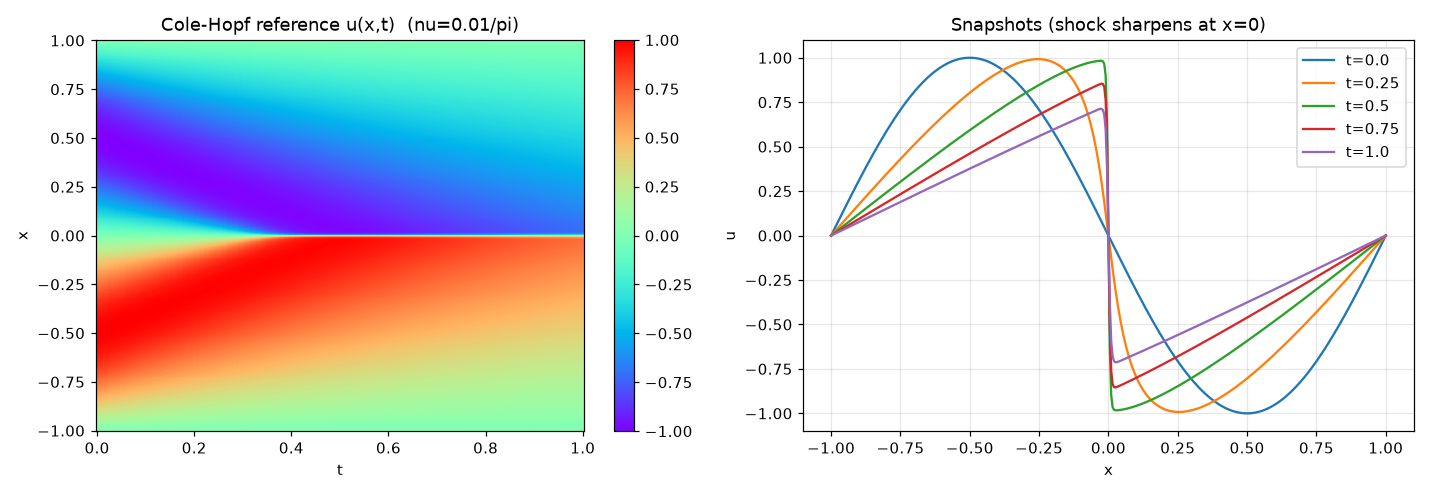
\includegraphics[width=0.85\textwidth]{burgers_reference.png}
  \caption{Cole--Hopf reference for viscous Burgers. Left: $u(x,t)$; right: snapshots
  showing the front forming at $x=0$.}
  \label{fig:reference}
\end{figure}

\subsection{Models}
\textbf{QAPINN}: $(x,t)\to\mathrm{VQC}\to$ classical post-network $\to u$. A fixed map
sends coordinate $i \bmod 2$ to qubit $i$ (no trainable pre-network, so the Fourier
band lives directly in $(x,t)$). The VQC has 4 qubits, $L$ layers of $R_Y$ angle
encoding with re-uploading, trainable rotations, a CNOT pattern (\emph{linear} chain
or \emph{none}), and $\langle Z_i\rangle$ readout. The small post-network is $[4,16,1]$
($L=3$: 24 quantum + 97 classical = 121 parameters); the larger one is $[4,32,32,1]$
(1273 parameters). All networks use $\tanh$.

\textbf{Controls} (Table~\ref{tab:models}): a \emph{parameter-matched} classical MLP;
a \emph{structural} control (CFE) that keeps the QAPINN's post-network but replaces
the VQC with a classical $\mathrm{Linear}(2\to4)+\tanh$ front end, so the only
difference is a quantum versus classical front end; and, at the larger scale, a
\emph{depth-matched} classical MLP with the same number of hidden layers as the
QAPINN counting the VQC as one, plus a \emph{balanced} two-layer MLP.

\begin{table}[t]
  \centering\small
  \begin{tabular}{lllr}
    \toprule
    Scale & Model & Architecture & Params \\
    \midrule
    \multirow{5}{*}{Small}
      & QAPINN, depth 3 (linear / none) & VQC(4q, $L{=}3$) $\to[4,16,1]$ & 121 \\
      & QAPINN, depth 5 (linear) & VQC(4q, $L{=}5$) $\to[4,16,1]$ & 137 \\
      & Classical & $[2,7,11,1]$ & 121 \\
      & CFE (structural) & Linear$(2{\to}4)$+tanh $\to[4,16,1]$ & 109 \\
    \midrule
    \multirow{6}{*}{Larger}
      & QAPINN, depth 3 (linear / none) & VQC(4q, $L{=}3$) $\to[4,32,32,1]$ & 1273 \\
      & CFE (structural) & Linear$(2{\to}4)$+tanh $\to[4,32,32,1]$ & 1261 \\
      & Classical, depth-matched & $[2,22,22,22,1]$ & 1101 \\
      & Classical, balanced & $[2,32,32,1]$ & 1185 \\
      & Classical, shallow & $[2,16,68,1]$ & 1273 \\
    \bottomrule
  \end{tabular}
  \caption{Models in the converged study. Small: Adam 2500 + L-BFGS 400 iterations,
  4000 interior points. Larger: Adam 3000 + L-BFGS 600, 6000 interior points. Both use
  learning rate $10^{-2}$ and 150 boundary/initial points, identical for every model.}
  \label{tab:models}
\end{table}

\subsection{Training, statistics and verification}
Every model at a given scale is trained under the identical protocol of
Table~\ref{tab:models}. Seeds $0$--$5$ are used where $n=6$ ($0$--$2$ where $n=3$).
We report mean $\pm$ sample standard deviation and two-sided Welch $t$-test $p$-values
(denoted $p$), computed from the per-run logs by a script in the repository; Student
and Mann--Whitney values are given there for comparison. The VQC is simulated with
PennyLane~\cite{pennylane} (\texttt{default.qubit}, exact statevector, backpropagation
for the second derivatives the residual needs).

Before any comparison we checked every load-bearing computation against an
independent reference (Appendix~\ref{app:verify}): autograd residuals against analytic
ones, derivatives against finite differences, the error metric on the exact solution,
parameter counts, and same-seed reproducibility. A one-qubit sweep confirms that the
VQC output contains no harmonic above the re-upload depth for $L=1,\dots,6$.

% ===========================================================================
\section{Results}
\subsection{Small scale: the classical PINN is best}\label{sec:small}
Table~\ref{tab:small} and Fig.~\ref{fig:seeds} (left) give the converged results at
$\sim$121 parameters. The classical MLP has the lowest mean error and is significantly
better than both depth-3 QAPINNs ($p=0.003$ against the linear-entanglement reference
design, $p=0.009$ against the unentangled variant). Increasing VQC depth to 5 lowers
the QAPINN's error to the level of the structural control ($p=0.99$); the gap to the
classical MLP is then not significant ($p=0.34$, $n=3$).

\begin{table}[t]
  \centering\small
  \begin{tabular}{lrcc}
    \toprule
    Model & Params & \relL{} (mean $\pm$ sd) & $n$ \\
    \midrule
    Classical $[2,7,11,1]$ & 121 & $\mathbf{0.248\pm0.038}$ & 3 \\
    QAPINN depth 5, linear & 137 & $0.314\pm0.090$ & 3 \\
    CFE (structural) & 109 & $0.315\pm0.032$ & 3 \\
    QAPINN depth 3, none & 121 & $0.379\pm0.035$ & 6 \\
    QAPINN depth 3, linear & 121 & $0.402\pm0.056$ & 6 \\
    \bottomrule
  \end{tabular}
  \caption{Converged results at small scale on Burgers.}
  \label{tab:small}
\end{table}

\begin{figure}[t]
  \centering
  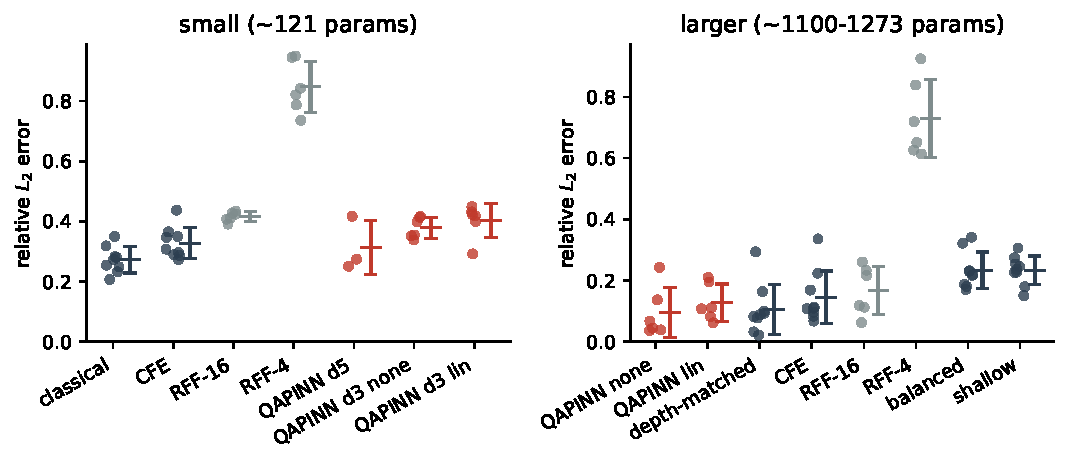
\includegraphics[width=\textwidth]{seeds.pdf}
  \caption{Per-seed relative $L_2$ error (dots) with mean $\pm$ sd (bars). Red: QAPINN; dark:
  classical models and controls. Left: small scale. Right: larger scale; the best QAPINN
  is separated from the shallow classical network but not from the depth-matched or
  structural controls, and seed-to-seed spread is large.}
  \label{fig:seeds}
\end{figure}

\subsection{Larger scale: the apparent advantage is architectural}\label{sec:large}
At the small scale every model still leaves the front partly unresolved
(\relL{} $0.25$--$0.40$). We therefore repeated the study at $\sim$1273 parameters,
where the best runs reach \relL{} $\approx0.03$--$0.04$ (Table~\ref{tab:large},
Fig.~\ref{fig:seeds}, right).

\begin{table}[t]
  \centering\small
  \begin{tabular}{lrcc}
    \toprule
    Model ($n=6$ each) & Params & \relL{} (mean $\pm$ sd) & vs QAPINN-none \\
    \midrule
    QAPINN depth 3, none & 1273 & $\mathbf{0.094\pm0.082}$ & --- \\
    QAPINN depth 3, linear & 1273 & $0.128\pm0.061$ & $p=0.44$ \\
    Classical, depth-matched & 1101 & $0.128\pm0.091$ & $p=0.51$ \\
    CFE (structural) & 1261 & $0.145\pm0.100$ & $p=0.36$ \\
    Classical, balanced & 1185 & $0.203\pm0.027$ & $p=0.021$ \\
    Classical, shallow & 1273 & $0.241\pm0.041$ & $p=0.005$ \\
    \bottomrule
  \end{tabular}
  \caption{Converged results at larger scale. $p$: two-sided Welch $t$-test against
  QAPINN-none.}
  \label{tab:large}
\end{table}

Against the shallow classical network alone, the QAPINN appears clearly better
($p=0.005$; this survives a Holm correction over the five comparisons, while the
balanced-network comparison, $p=0.021$, does not). Against the two fair controls it is
not: a depth-matched classical MLP with \emph{fewer} parameters and the structural
control are both statistically indistinguishable from it. The advantage over the
shallow network is therefore attributable to depth and post-network shape, which a
classical model reproduces, rather than to the quantum layer.

This is a failure to reject, not a demonstration of equality. Seed-to-seed spread
($\mathrm{sd}\approx0.08$--$0.10$) exceeds the mean differences ($\approx0.03$--$0.05$),
so the comparison is under-powered. One QAPINN-none seed ($0.243$) is an outlier;
removing it lowers the mean but the comparison with the depth-matched control remains
non-significant ($p=0.17$).

\subsection{Entanglement has no detectable effect}\label{sec:ent}
With three seeds at small scale, the unentangled QAPINN looked better than the linear
one ($0.369$ vs $0.424$; Student $p=0.024$, Welch $p=0.060$). Extending to six seeds
removed the effect ($0.379$ vs $0.402$, $p=0.42$); one of the new linear seeds
($0.292$) is the best depth-3 run. At the larger scale the difference is also not
significant ($0.094$ vs $0.128$, $p=0.44$). Earlier single-seed ablations with four
entanglement patterns (Appendix~\ref{app:prelim}) likewise showed entanglement entropy
varying widely with no corresponding change in error.

\subsection{Error is governed by output bandwidth}\label{sec:spectral}
For every trained model we computed the spatial spectrum of $u_\theta$ on the
evaluation grid (magnitude of the FFT along $x$, averaged over $t$) and its 99\%-energy
bandwidth $K_{99}$: the smallest $K$ such that harmonics $1,\dots,K$ hold 99\% of the
non-constant spectral energy. The reference has $K_{99}=13$.

\begin{figure}[t]
  \centering
  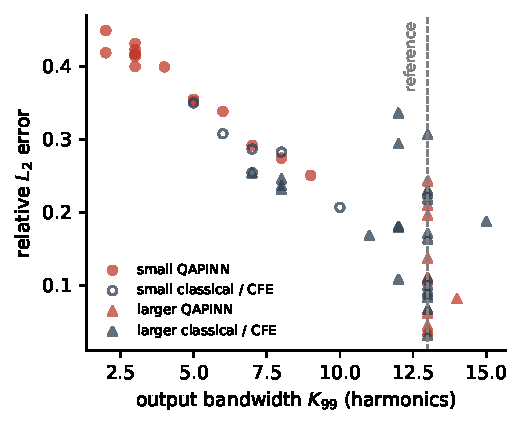
\includegraphics[width=0.55\textwidth]{bandwidth.pdf}
  \caption{Relative $L_2$ error against the realised output bandwidth $K_{99}$ for all 57
  converged models (circles: small scale; triangles: larger scale; red: QAPINN). The
  dashed line is the reference bandwidth.}
  \label{fig:bandwidth}
\end{figure}

Figure~\ref{fig:bandwidth} shows a single trend across model families (Spearman
$\rho=-0.85$, $p<10^{-16}$, $n=57$). Within the small QAPINNs the relation is
nearly deterministic ($\rho=-0.94$, $n=15$): depth-3 QAPINNs mostly realise
$K_{99}=2$--$6$, while the small classical MLPs reach $7$--$10$ and the structural
control $5$--$7$. The one depth-3 seed that reaches $K_{99}=7$ is also the most
accurate. At the larger scale every QAPINN, structural control and depth-matched
network reaches $K_{99}=11$--$14$ (some shallow and balanced classical runs stay at
7--8). Bandwidth then explains much less of the error ($\rho=-0.49$, $n=36$): models at
the reference bandwidth still range from 0.03 to 0.34, a spread set by how well each
seed's optimisation resolves the front rather than by which frequencies are present.

This corrects a claim in our own earlier analysis. The VQC's \emph{features} are
band-limited by construction. With $R_Y(x)$ encoding, $L=3$ and two of the four qubits
encoding $x$, each readout of a trained unentangled QAPINN contains angular frequencies
in $x$ up to 3; with the linear CNOT chain, which mixes the two $x$-qubits, the readouts
reach 4--6 (measured exactly, since the features are $2\pi$-periodic in $x$). Either way
this is at most about two periods across $[-1,1]$, far below the 13 harmonics the
reference needs. The
\emph{model} is not: the $\tanh$ post-network forms products of features and so can
synthesise higher harmonics. Whether it does depends on its capacity. The small
post-network mostly fails to; the larger one always succeeds. The band set by VQC depth
is therefore a soft constraint on small models, not a property of the QAPINN as such.

\subsection{Encoding scale}
In a single-seed preliminary sweep (Appendix~\ref{app:prelim}) the input scale of the
encoding had an optimum near 1. At scale $2\pi$ the model collapsed to the trivial
solution $u\equiv0$ (\relL{} $=1.000$), which satisfies the boundary conditions but not
the initial condition. With scale $2\pi$ each re-upload wraps the domain twice, so
nearby collocation points map to distant circuit states; we suggest this as the cause
but did not test it further.

% ===========================================================================
\section{Interpretation}\label{sec:why}
We mark each explanation as \emph{measured} (directly supported by our data) or
\emph{reasoned} (consistent with theory and our controls but not isolated).

\paragraph{The quantum layer is a fixed low-frequency feature map (measured).} With raw
coordinates as input and $L=3$, the VQC supplies the post-network with trigonometric
features of bounded frequency. Error tracks how far the post-network can extend that
band (Section~\ref{sec:spectral}). A classical front end of the same width gives the
post-network features that are at least as useful: the structural control is better
than or statistically indistinguishable from the QAPINN at both scales.

\paragraph{Why there is no quantum-specific advantage (reasoned).} The representational
work is done by the classical post-network, which sits downstream of the quantum layer.
A front end only needs to supply features from which the post-network can build the
solution. Burgers' solution is low-frequency away from the front and needs many
harmonics at the front; the VQC's band offers no shortcut to the latter, so any front
end of comparable richness performs similarly. This is the same reason classical
Fourier-feature front ends~\cite{tancik} help only when their frequencies match the
target.

\paragraph{Why entanglement is neutral (partly measured).} Entanglement does change the
features: the linear CNOT chain doubles the highest $x$-frequency of the readouts from 3
to 6 (Section~\ref{sec:spectral}) and redistributes which coefficients are
reachable~\cite{mhiri}. Yet it has no detectable effect on error. Our interpretation is
that both changes are redundant once a post-network follows: products of the
unentangled per-qubit features already contain these sum frequencies, and the
post-network forms such products itself. We tried to measure the
mechanism directly (per-qubit feature correlation and effective rank, with and without
entanglement) and the two measures disagreed, so we report this as an interpretation
consistent with the null result.

\paragraph{Why the front defeats small models (partly measured).} The front's Fourier
content decays slowly with $k$, and gradient-trained networks fit high frequencies
last~\cite{xu,rahaman}. For the larger QAPINNs where training-time spectra were logged,
the order in which harmonics reach half their initial error correlates positively with
$k$ in 6 of 8 runs (Spearman $\rho$ from $-0.16$ to $0.84$), weak support for this
classical explanation. The quantum layer neither causes nor removes it.

% ===========================================================================
\section{A protocol for evaluating QAPINN claims}\label{sec:protocol}
Three positive findings appeared during this project and were removed by later checks:
(i) a larger diversity of post-network neurons with a quantum front end, which
disappeared against the structural control (Appendix~\ref{app:prelim}); (ii) an
entanglement effect at $n=3$, which disappeared at $n=6$
(Section~\ref{sec:ent}); and (iii) an advantage at larger scale, which disappeared
against a depth-matched classical network (Section~\ref{sec:large}). A fourth reading,
that VQC depth caps the model at a fixed low band, holds for the features and loosely
for small models, but not for models with a larger post-network
(Section~\ref{sec:spectral}). Each of the first three would have been reported as
positive without the corresponding check:
\begin{enumerate}[nosep]
  \item \textbf{Converge.} Train with a second-order optimiser (here L-BFGS) after Adam.
  Without it, every Burgers model in our preliminary runs stalled at
  \relL{} $0.42$--$0.59$ and the differences between them were within seed noise.
  \item \textbf{Use fair controls.} Compare against a parameter-matched, a structurally
  matched and a depth-matched classical network, all trained under the same protocol.
  \item \textbf{Require multi-seed significance.} Use at least six seeds, report the
  test used, and treat $n=3$ effects as provisional.
  \item \textbf{Separate features from model.} Test Fourier-band claims on the VQC output
  and on the trained model separately.
\end{enumerate}
An advantage that passes all four checks would justify a circuit-design methodology.
None of ours did.

% ===========================================================================
\section{Limitations}
\begin{enumerate}[nosep]
  \item \textbf{Statistical power.} With $n\le6$ and seed spread of $\sim$0.08, the
  decisive comparisons are failures to reject. Same-seed reruns that include L-BFGS
  are not bit-identical across machines, which adds variance. More seeds would tighten
  the null results.
  \item \textbf{Scope.} One nonlinear PDE in one spatial dimension (plus heat as a
  sanity check), two model scales, 4-qubit circuits, and $R_Y$ encoding of raw
  coordinates. A lid-driven cavity case is implemented in the code but was not run.
  Other encodings, larger circuits or other PDEs could behave differently.
  \item \textbf{Simulation only.} Exact statevector simulation without shot noise or
  hardware noise, which would only add difficulties for the quantum model. Fewer
  parameters do not mean lower cost: QAPINN training took roughly 130--500 times longer in
  wall-clock time than the classical models (CPU laptops).
  \item \textbf{Untested mechanisms.} The explanations marked \emph{reasoned} in
  Section~\ref{sec:why} were not isolated experimentally, and the encoding-scale
  collapse is a single-seed observation.
\end{enumerate}

% ===========================================================================
\section{Conclusion}
On 1-D Burgers' equation, with converged training, multi-seed statistics and fair
classical controls, we find no quantum-specific advantage for QAPINNs: at small scale
the classical PINN is best, and at larger scale the QAPINN ties both a depth-matched
classical network and a structural control. Entanglement has no detectable effect. A
spectral analysis of all trained models shows why: error is governed by the bandwidth
the model realises, the VQC contributes a fixed low-frequency feature map, and the
classical post-network determines whether that band is extended. Whether an advantage
appears on other PDEs, encodings or scales remains open; the protocol in
Section~\ref{sec:protocol} is a way to test such a claim.

\section*{Code and data availability}
Code, configurations, per-run logs and metrics, and the trained weights of the
converged models are available at\\ \url{https://github.com/hementhu/qapinn-bqp}. The scripts
\texttt{compute\_stats.py}, \texttt{verify\_claims.py} and \texttt{verify\_pipeline.py}
regenerate every statistic, spectral measurement and verification check reported here.

\section*{Acknowledgements}
This work began as a submission to the BQP industry challenge of the WISER Global
Quantum+AI Program 2026. The author used Claude Code (Anthropic) to help implement
the code, run and aggregate experiments, search the literature, audit results and
draft text. The author directed the research questions and experiments, checked the
results, and takes responsibility for the content.

% ===========================================================================
\begin{thebibliography}{99}
\small
\bibitem{raissi} M.~Raissi, P.~Perdikaris, G.~E.~Karniadakis. Physics-informed neural
  networks: A deep learning framework for solving forward and inverse problems involving
  nonlinear partial differential equations. \emph{J.\ Comput.\ Phys.}\ \textbf{378},
  686--707 (2019).
\bibitem{qapinn} J.~Shah, R.~Lineswala, A.~Chopra. Benchmarking quantum-assisted
  physics-informed neural networks (QA-PINN) for computational fluid dynamics.
  \emph{IEEE International Conference on Quantum Computing and Engineering (QCE)}
  (2024). \textcolor{red}{[VENUE/DOI TO CONFIRM]}
\bibitem{qcpinn} A.~Farea, S.~Khan, M.~S.~Celebi. QCPINN: Quantum-classical
  physics-informed neural networks for solving PDEs. arXiv:2503.16678 (2025).
\bibitem{schuld} M.~Schuld, R.~Sweke, J.~J.~Meyer. Effect of data encoding on the
  expressive power of variational quantum-machine-learning models. \emph{Phys.\ Rev.\ A}
  \textbf{103}, 032430 (2021).
\bibitem{reupload} A.~P\'erez-Salinas, A.~Cervera-Lierta, E.~Gil-Fuster, J.~I.~Latorre.
  Data re-uploading for a universal quantum classifier. \emph{Quantum} \textbf{4}, 226
  (2020).
\bibitem{mhiri} H.~Mhiri, L.~Monbroussou, M.~Herrero-Gonz\'alez, S.~Thabet, E.~Kashefi,
  J.~Landman. Constrained and vanishing expressivity of quantum Fourier models.
  \emph{Quantum} \textbf{9}, 1847 (2025).
\bibitem{mcclean} J.~R.~McClean, S.~Boixo, V.~N.~Smelyanskiy, R.~Babbush, H.~Neven.
  Barren plateaus in quantum neural network training landscapes. \emph{Nat.\ Commun.}\
  \textbf{9}, 4812 (2018).
\bibitem{xu} Z.-Q.~J.~Xu, Y.~Zhang, T.~Luo, Y.~Xiao, Z.~Ma. Frequency principle:
  Fourier analysis sheds light on deep neural networks. \emph{Commun.\ Comput.\ Phys.}\
  \textbf{28}, 1746--1767 (2020).
\bibitem{rahaman} N.~Rahaman, A.~Baratin, D.~Arpit, F.~Draxler, M.~Lin, F.~Hamprecht,
  Y.~Bengio, A.~Courville. On the spectral bias of neural networks. \emph{ICML} (2019).
\bibitem{wang} S.~Wang, Y.~Teng, P.~Perdikaris. Understanding and mitigating gradient
  flow pathologies in physics-informed neural networks. \emph{SIAM J.\ Sci.\ Comput.}\
  \textbf{43}, A3055--A3081 (2021).
\bibitem{krishnapriyan} A.~S.~Krishnapriyan, A.~Gholami, S.~Zhe, R.~M.~Kirby,
  M.~W.~Mahoney. Characterizing possible failure modes in physics-informed neural
  networks. \emph{NeurIPS} (2021).
\bibitem{tancik} M.~Tancik, P.~P.~Srinivasan, B.~Mildenhall, S.~Fridovich-Keil,
  N.~Raghavan, U.~Singhal, R.~Ramamoorthi, J.~T.~Barron, R.~Ng. Fourier features let
  networks learn high frequency functions in low dimensional domains. \emph{NeurIPS}
  (2020).
\bibitem{dqc} O.~Kyriienko, A.~E.~Paine, V.~E.~Elfving. Solving nonlinear differential
  equations with differentiable quantum circuits. \emph{Phys.\ Rev.\ A} \textbf{103},
  052416 (2021).
\bibitem{chen} Chen, Shaviner, Chandravamsi, Pisnoy, Frankel, Pereg. Quantum
  physics-informed neural networks for Maxwell's equations. arXiv:2506.23246 (2025).
\bibitem{pennylane} V.~Bergholm et al. PennyLane: Automatic differentiation of hybrid
  quantum-classical computations. arXiv:1811.04968 (2018).
\end{thebibliography}

% ===========================================================================
\appendix
\section{Pipeline verification}\label{app:verify}
\begin{table}[h]
  \centering\small
  \begin{tabular}{lll}
    \toprule
    Check & Method & Result \\
    \midrule
    Burgers residual & autograd vs analytic $u_t+uu_x-\nu u_{xx}$ & max error $1.2\times10^{-7}$ \\
    Heat residual & exact solution & max $|r|$ $1.2\times10^{-7}$ \\
    Derivative & autograd vs finite differences & agree to $2\times10^{-4}$ \\
    VQC bandwidth & 1-qubit sweep, max harmonic vs $L$ & equal for $L=1,\dots,6$ \\
    Error metric & \relL{} of the exact solution & $4.0\times10^{-8}$ \\
    Parameter matching & the four base configurations & all 121 \\
    Reproducibility & same seed, Adam-only run & bit-identical \\
    \bottomrule
  \end{tabular}
  \caption{Correctness checks (\texttt{verify\_pipeline.py}, \texttt{verify\_claims.py}).}
\end{table}

\section{Preliminary single-seed ablations}\label{app:prelim}
Before the converged study we ran one-factor ablations with Adam only (2000 iterations,
1500 collocation points, seed 0). These runs are undertrained: every Burgers model has
\relL{} between $0.42$ and $0.59$ (except the collapsed $2\pi$ run), and the
differences below are within the seed spread we later measured. They are reported for
completeness; none of the comparisons is used as evidence in the main text. The classical
reference in this table is a $[2,30,1]$ MLP sized to each QAPINN's parameter count,
which differs from the $[2,7,11,1]$ network of Table~\ref{tab:small}.

\begin{table}[h]
  \centering\small
  \begin{tabular}{llccc}
    \toprule
    Factor & Setting & Params & QAPINN & Classical \\
    \midrule
    \multirow{4}{*}{Depth $L$} & 1 & 105 & 0.572 & 0.522 \\
      & 2 & 113 & 0.493 & 0.502 \\
      & 3 (base) & 121 & 0.472 & 0.535 \\
      & 5 & 137 & 0.424 & 0.500 \\ \midrule
    \multirow{4}{*}{Entanglement} & none & 121 & 0.456 & 0.535 \\
      & linear (base) & 121 & 0.472 & 0.535 \\
      & ring & 121 & 0.485 & 0.535 \\
      & all-to-all & 121 & 0.488 & 0.535 \\ \midrule
    \multirow{4}{*}{Post-network} & none (linear) & 29 & 0.544 & 0.533 \\
      & $[8]$ & 73 & 0.478 & 0.533 \\
      & $[32]$ & 217 & 0.466 & 0.505 \\ \midrule
    \multirow{3}{*}{Qubits} & 3 & 99 & 0.501 & 0.470 \\
      & 5 & 143 & 0.468 & 0.541 \\
      & 6 & 165 & 0.443 & 0.465 \\ \midrule
    \multirow{2}{*}{Readout} & single $\langle Z_0\rangle$ & 73 & 0.591 & 0.533 \\
      & $ZZ$ correlators & 169 & 0.472 & 0.515 \\ \midrule
    \multirow{3}{*}{Input scale} & 0.5 & 121 & 0.513 & 0.535 \\
      & $\pi$ & 121 & 0.516 & 0.535 \\
      & $2\pi$ & 121 & 1.000 & 0.535 \\
    \bottomrule
  \end{tabular}
  \caption{Preliminary ablations on Burgers (\relL{}, single seed, undertrained).}
\end{table}

\begin{figure}[h]
  \centering
  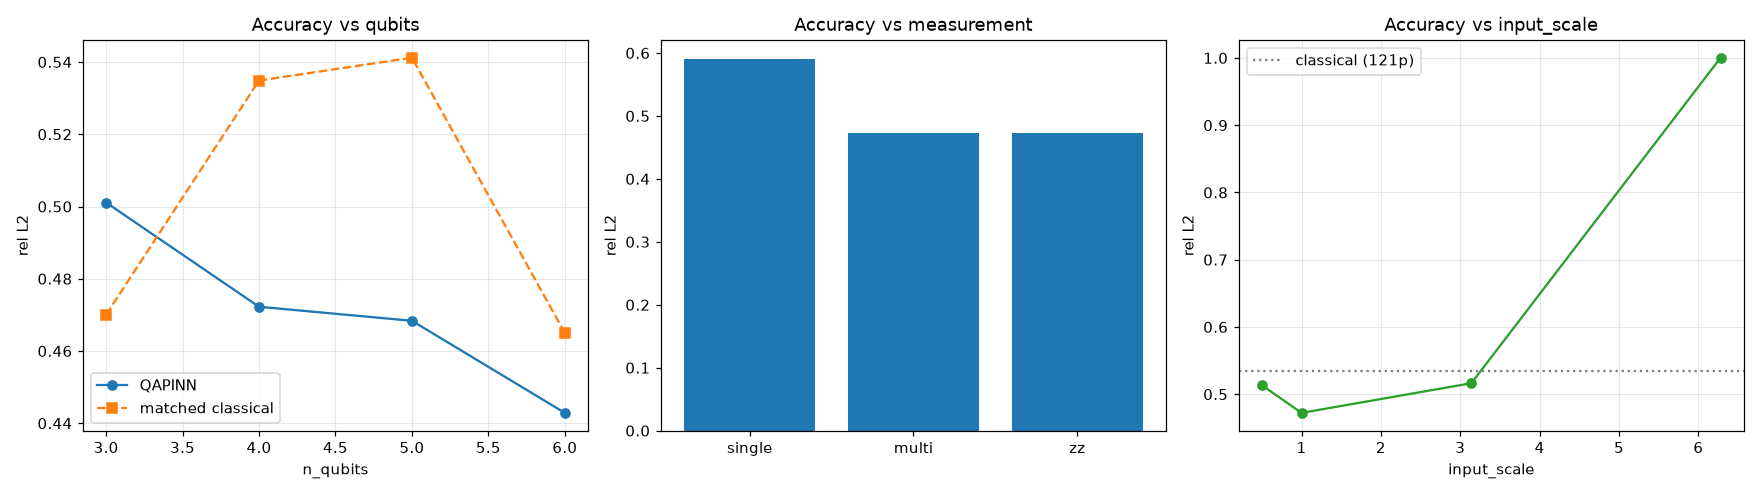
\includegraphics[width=\textwidth]{tier3_sweeps.png}
  \caption{Preliminary sweeps over qubit count, readout and input scale (single seed,
  undertrained). The input-scale panel shows the collapse at $2\pi$.}
\end{figure}

\paragraph{Front-end comparison.} Against a plain classical PINN of a different shape, the
quantum front end appeared to make the post-network neurons about twice as diverse
(normalised effective rank) and to increase post-network gradient variance. Against the
structural control, which uses the identical post-network, neither effect was
consistent: diversity was higher with the classical front end along the depth axis and
with the quantum front end along the qubit axis, and the gradient-variance difference
reversed at 5--6 qubits. We therefore do not claim either effect.

\end{document}
